\vspace{-4px}
\section{Learning@home}\label{sect:method}
\vspace{-2px}

Our main idea is to use the existing properties of mixture-of-experts and distributed hash tables to work around the limitations of volunteer computing. We begin with a method for distributed training of MoE layers, then extend it to provide fault tolerance and decentralized bookkeeping.

\vspace{-2px}
\subsection{Decentralized Mixture-of-Experts}\label{sect:method_dmoe}
\vspace{-2px}

The fundamental building block of our approach is Decentralized Mixture-of-Experts (DMoE) --- a layer that contains multiple independent ``expert'' sub-networks distributed over a pool of workers. In addition to experts, each worker has a gating function: a lightweight sub-network that selects experts depending on the input. Similarly to regular mixture-of-experts, DMoE is a general-purpose layer that can process any input type by using the appropriate experts (e.g., convolutional or attentive).

Workers within the DMoE layer interact using Kademlia DHT protocol (Section \ref{sect:related_dht}). This DHT stores metadata, such as expert weights and worker status. Figure \ref{fig:dmoe_inference} explains DMoE inference:

\begin{figure}[h]
\vspace{-10px}
    \centering
    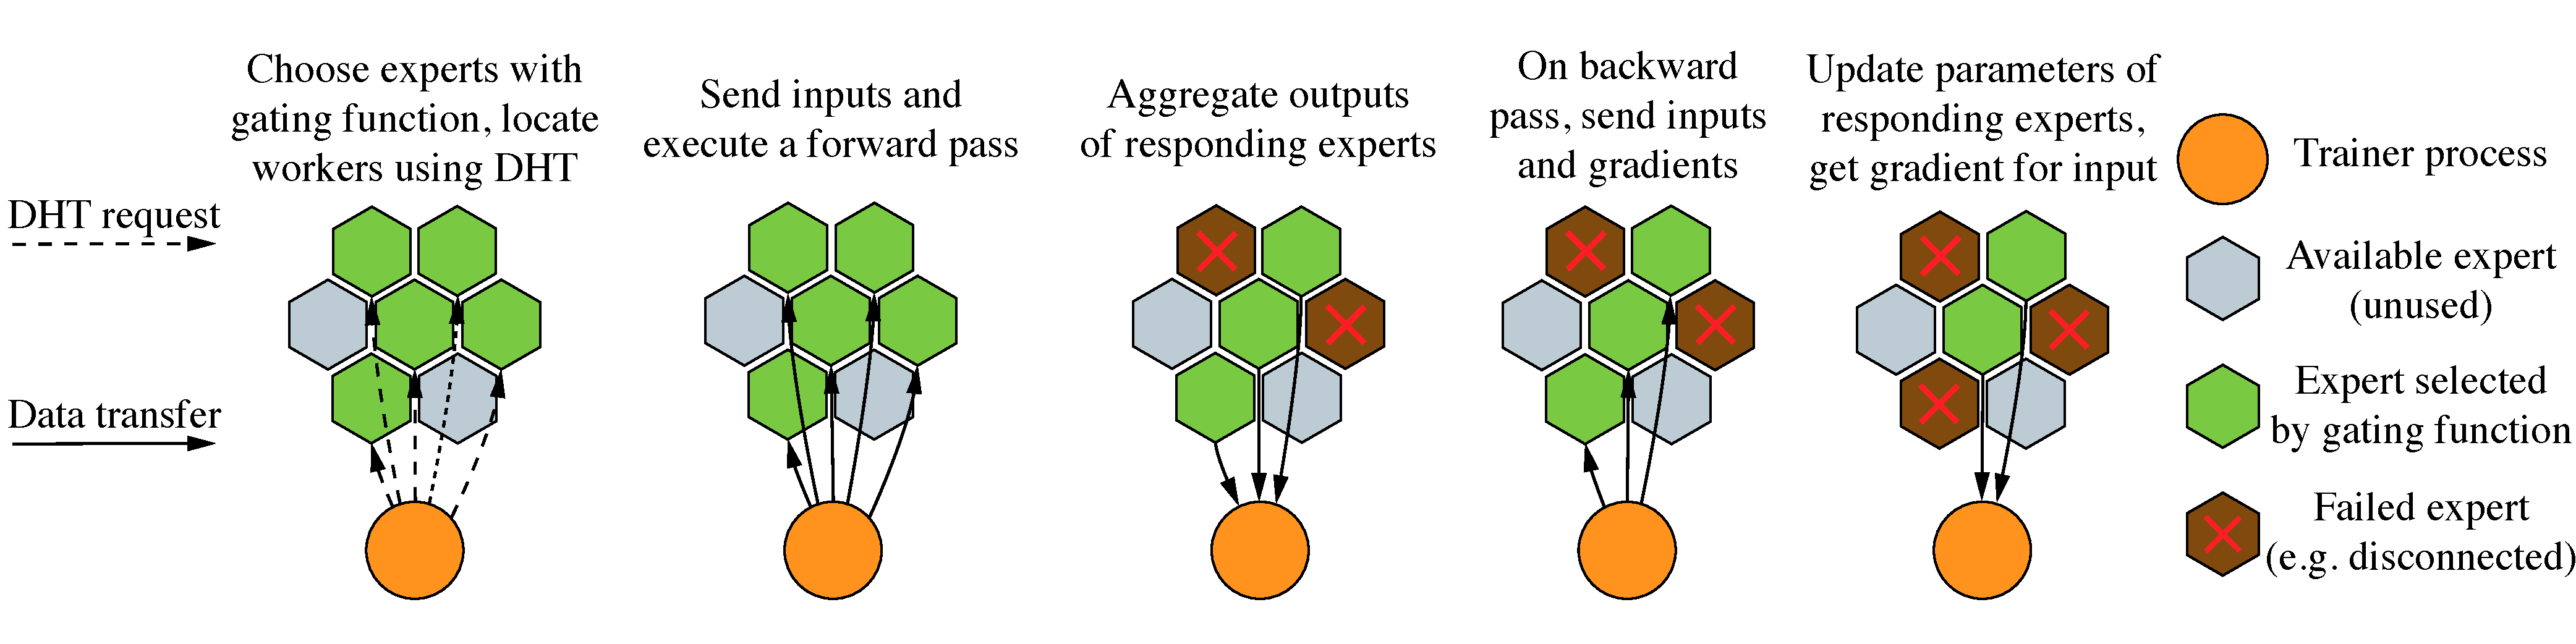
\includegraphics[width=400px,height=100px]{resources/schematic-training-v2.pdf}
    \caption{Forward and backward passes for Decentralized Mixture of Experts.}
    \label{fig:dmoe_inference}
\end{figure}

\vspace{-4px}


This procedure takes at most $O(k \log N)$ DHT queries to locate the chosen experts and $k$ direct interactions with these experts to do the actual processing. As long as $k~\ll~N$, we can increase the total number of experts without compromising the inference speed. Furthermore, we argue that DMoE layers automatically solve most of the issues that arise in the volunteer computing scenario.

\textbf{Fault tolerance.} If some of the $k$ chosen experts fail to respond due to a hardware or network error, DMoE can exclude those experts from averaging. The effect of such exclusion is similar to using Dropout  \cite{srivastava2014dropout} with regular mixture-of-experts. As a side effect, training DMoE on a faulty infrastructure will automatically adapt the mixture to the failure points of that infrastructure.

\textbf{Volunteer hardware.} Compute nodes can serve different numbers of experts based on their hardware capabilities. If one node leaves the network, another can take its place by retrieving the latest expert checkpoints from the DHT.

\textbf{Load balancing.} Mixture-of-experts layers can be regularized to balance the rate at which they select each expert in the mixture \cite{shazeer2017outrageously, pkm}. Originally designed to improve MoE quality, this regularization has a side-effect of improving resource utilization by balancing computation load between workers.

\textbf{Asynchronous training.} Due to communication latency in distributed systems, a single input can take a long time to process. The traditional solution is to train asynchronously \cite{volunteer_dl_async}. Instead of waiting for the results on one training batch, a worker can start processing the next batch right away. This approach can significantly improve hardware utilization at the cost of stale gradients. 

Fortunately, Mixture-of-Experts accumulates staleness at a slower pace than regular neural networks. Only a small subset of all experts processes a single input; therefore, two individual inputs are likely to affect completely different experts. In that case, updating expert weights for the first input will not introduce staleness for the second one.
We elaborate on this claim in Section \ref{sect:exp_convergence}.

\vspace{-3px}
\subsection{Structured Gating Function}\label{sect:method_gating}
\vspace{-2px}

Since DMoE can use up to millions of experts, the gating function can no longer iterate over each expert in the mixture. Furthermore, the nodes in such a system are continually joining and leaving. Consequently, the expert selection procedure cannot rely on the availability of any individual node.

\vspace{-1px}

With this in mind, we propose a gating function inspired by product key layers~\cite{pkm}. First, we organize experts into a $d$-dimensional grid. Each expert $f$ is associated with a unique tuple of integers: $\textrm{uid}(f) = (u_0, u_1, \ldots, u_{d-1}), u_i \in [0, M)$. The grid dimensions $d, M$ should be chosen to accommodate all experts with some level of redundancy. Having extra grid space allows DMoE to allocate additional experts midway through training if more volunteers join. %

\vspace{-1px}

The gating function itself consists of $d$ linear layers $g_0,\dots\,g_{d-1}$ and computes expert priority in an additive manner: $g(x, f) = \sum_{i=0}^{d - 1} g_i(x)[u_i]$. Such a function only needs to predict $d$ vectors of size $M$, which makes it significantly easier to compute and send over the network. Furthermore, this gating function can choose top-$k$ highest-scoring experts in logarithmic time (see Appendix B, C).

\vspace{-4px}

After choosing the appropriate experts, a worker should find their respective servers (in $O(k \log N)$ time using DHT) and pass the input vector for processing (see Figure \ref{fig:teaser}). Once all the experts have finished processing, the worker aggregates expert outputs by weighted averaging:
\begin{equation}
\label{eq:dmoe_averaging}
    \textrm{DMoE}(x) = \!\!\!\!\!\! \sum_{f \in \mathrm{TopK}(x)} \!\!\!\!\!\! f(x) \frac{\exp\left({g(x, f)}\right)}{\sum_{f' \in \mathrm{TopK}(x)} \exp\left({g(x, f')}\right)}
    \space\text{ , $\mathrm{TopK}(x)$ are $k$ best experts w.r.t. $g$}
\end{equation}
\vspace{-8px}

If some of the chosen experts have crashed or taken too long to perform the computation, we can exclude them from averaging and renormalize weights so that they still add up to 1. Trained with this exclusion policy, DMoE will learn experts with overlapping specializations that are more resistant to individual node failure.
\vspace{-4px}
\subsection{Training infrastructure}\label{sect:method_athome}
\vspace{-2px}

Finally, we describe Learning@home --- a deep learning infrastructure that performs distributed training of large models on hardware provided by volunteers. Each worker runs three components:

\begin{figure}[h!]
\vspace{-6px}
    \begin{minipage}{0.45\linewidth}
    \begin{itemize}[leftmargin=*]
        \item \textbf{Trainer} --- forming batches and training;
        \item \textbf{Runtime} --- inference and expert updates;
        \item \textbf{DHT Node} --- bookkeeping and routing;
    \end{itemize}\end{minipage}\begin{minipage}{0.55\linewidth}
        \centering\raisebox{\dimexpr \topskip-\height}{
        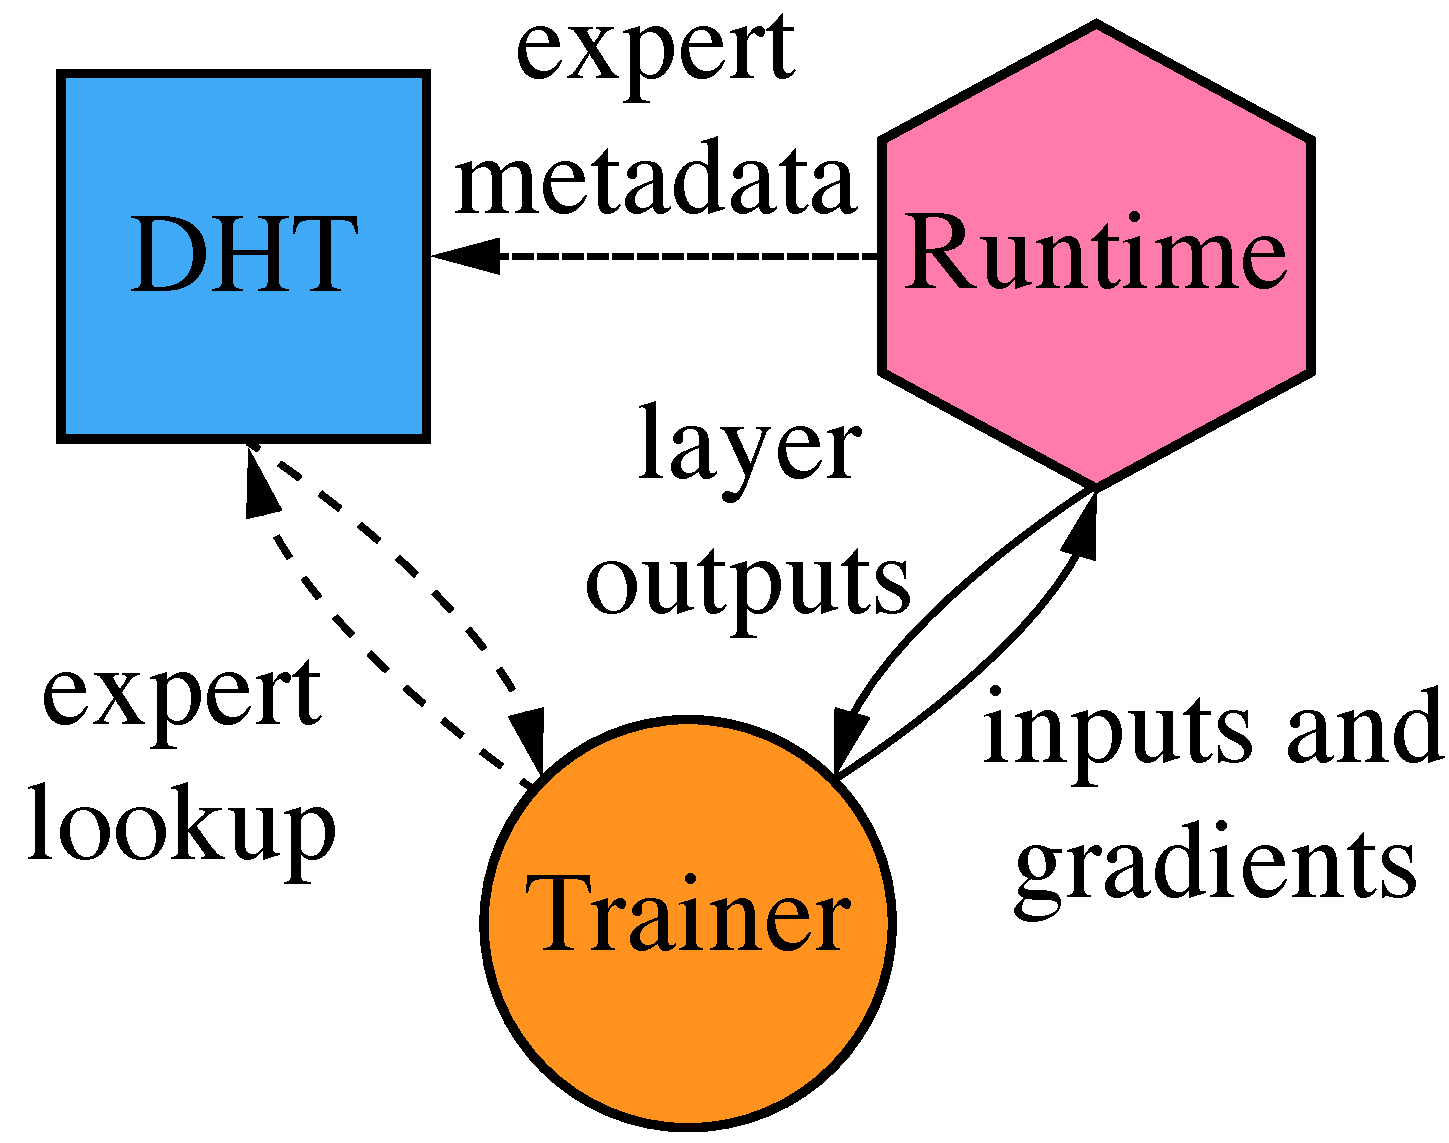
\includegraphics[width=90px]{resources/l_at_home.pdf}}
    \end{minipage}
    \caption{Learning@home components and their interaction.}
    \vspace{-12pt}
    \label{fig:dmoe}
\end{figure}


\textbf{Trainer} generates batches and propagates them through the model. After forming a batch and converting it into an input vector, the trainer iterates over a sequence of DMoE layers and organizes forward and backward passes, as described in Sections \ref{sect:method_dmoe} and \ref{sect:method_gating}. Learning@home fully embraces the asynchronous training paradigm, where a trainer can process hundreds of concurrent batches.

\vspace{-1px}

\textbf{Runtime} is responsible for expert inference and training. This is the only process that has access to participant's GPU device(s). Once all the experts are initialized, runtime listens to the incoming connections from trainers and handles two types of requests:
\vspace{-4px}
\begin{itemize}[leftmargin=*]
    \item \textbf{Forward}: given inputs, compute and return expert outputs on these inputs (no side-effects);
    \item \textbf{Backward}: given inputs and gradients of loss function w.r.t. outputs, return gradients w.r.t. inputs and \textit{update expert parameters by gradient descent}.
\end{itemize}
\vspace{-4px}

Since trainers can operate under latency, the runtime is not required to process all requests right away. Instead, it aggregates requests into batches for better GPU utilization.

\vspace{-1px}

The runtime process relies on gradient checkpointing to avoid storing intermediate expert activations \cite{gradient_checkpointing_autograd,gradient_checkpointing_dl}.
This choice means that the expert $f_i(x)$ is called both during the forward and the backward passes.
We elaborate on the role of gradient checkpointing in Appendix D.

\vspace{-1px}

\textbf{DHT Node.} The final component of Learning@home infrastructure is a DHT for bookkeeping. For simplicity, we use unmodified Kademlia protocol\footnote{In particular, publicly available Kademlia implementation from \url{github.com/bmuller/kademlia}}, leaving further investigation to future work.

\vspace{-1px}

Each runtime periodically announces its experts to the DHT, associating their identifiers with the address of that runtime and the current timestamp (details in Appendix C). Trainers can then use those entries to find the workers responsible for the chosen experts. In addition to timestamps, a runtime also regularly saves latest expert weights into the same DHT for persistence. The resulting infrastructure becomes elastic and fault-tolerant as long as it has enough active participants.




